\section{Methods and results}\label{sec:methods_results}

\subsection{Sequential}

TODO: Algorithm description, variants, method description, other methods are only necessary modification of this method

TODO: Accumulator difference (one pixel differs - float64 vs float32) - single figure with 4 differences referred to later

TODO: Results, C++ as reference

TODO: Notice Firefox optimization after 5th run and chrome overall better optimization



\begin{figure}
    \groupBenchmark{
        \plotBenchmark{cpp_theta_SHT_Simple.csv}{cppColor}{{}}
        \addlegendentry{C++}

        \plotBenchmark{js-sequential_theta_SHT_Simple_node.csv}{nodeColor}{{}}
        \addlegendentry{Node}

        \plotBenchmark{js-sequential_theta_SHT_Simple_deno.csv}{denoColor}{{}}
        \addlegendentry{Deno}

        \plotBenchmark{js-sequential_theta_SHT_Simple_Firefox.csv}{firefoxColor}{{}}
        \addlegendentry{Firefox}

        \plotBenchmark{js-sequential_theta_SHT_Simple_Chrome.csv}{chromeColor}{{}}
        \addlegendentry{Chrome}

    } {
        \plotBenchmark{cpp_theta_SHT_Simple_Lookup.csv}{cppColor}{{}}
        \addlegendentry{C++}

        \plotBenchmark{js-sequential_theta_SHT_Simple_Lookup_node.csv}{nodeColor}{{}}
        \addlegendentry{Node}

        \plotBenchmark{js-sequential_theta_SHT_Simple_Lookup_deno.csv}{denoColor}{{}}
        \addlegendentry{Deno}

        \plotBenchmark{js-sequential_theta_SHT_Simple_Lookup_Firefox.csv}{firefoxColor}{{}}
        \addlegendentry{Firefox}

        \plotBenchmark{js-sequential_theta_SHT_Simple_Lookup_Chrome.csv}{chromeColor}{{}}
        \addlegendentry{Chrome}
    } {
        \plotBenchmark{cpp_theta_CHT_Simple.csv}{cppColor}{{}}
        \addlegendentry{C++}

        \plotBenchmark{js-sequential_theta_CHT_Simple_node.csv}{nodeColor}{{}}
        \addlegendentry{Node}

        \plotBenchmark{js-sequential_theta_CHT_Simple_deno.csv}{denoColor}{{}}
        \addlegendentry{Deno}

        \plotBenchmark{js-sequential_theta_CHT_Simple_Firefox.csv}{firefoxColor}{{}}
        \addlegendentry{Firefox}

        \plotBenchmark{js-sequential_theta_CHT_Simple_Chrome.csv}{chromeColor}{{}}
        \addlegendentry{Chrome}
    }
    [3400][850][14]
    \caption{Wyniki pomiarów czasu wydajności dla wykonania sekwencyjnego SHT i CHT.}
    \label{plot:sequential}
\end{figure}


TODO: Performance from devtools, show times in Math.sin and Math.cos

\begin{figure}
    \begin{subfigure}{0.29\textwidth}
        
\includegraphics[width=\linewidth] {../../packages/js-benchmarks/img/diff_seq_seq_lookup.png}
        \caption{Sequential \textit{LUT}}\label{fig:diff:seq_lut}
    \end{subfigure}\hfill
    \begin{subfigure}{0.29\textwidth}
        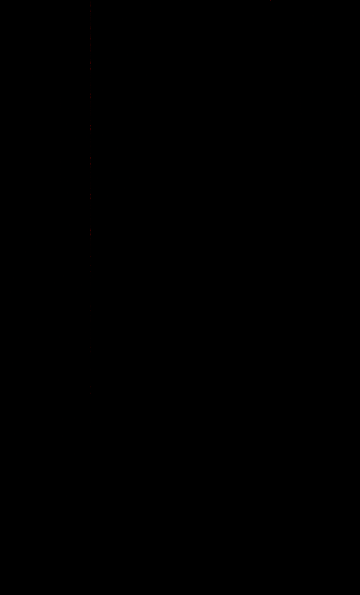
\includegraphics[width=\linewidth] {../../packages/js-benchmarks/img/diff_seq_wasm.png}
        \caption{WASM}\label{fig:diff:wasm}
    \end{subfigure}\hfill
    \begin{subfigure}{0.29\textwidth}
        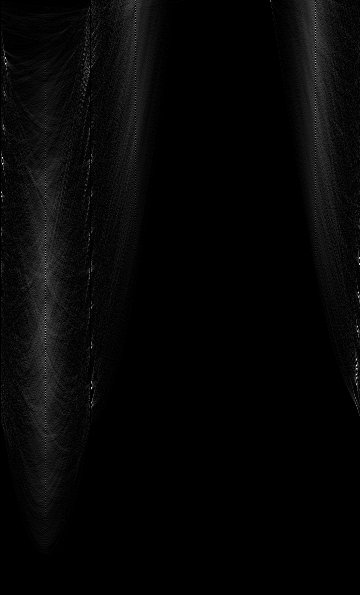
\includegraphics[width=\linewidth] {../../packages/js-benchmarks/img/diff_seq_gpu.png}
        \caption{WebGL}\label{fig:diff:gpu}
    \end{subfigure}
    \caption{Normalized absolute accumulator difference from sequential \textit{non-LUT} variant. Note the two-pixel difference in the upper right corner for Sequential \textit{LUT}.}\label{fig:diff}
\end{figure}


\subsection{Node C++ addon}

TODO: Method description, building process

TODO: Results, C++ and Sequential as reference



\begin{figure}
    \groupBenchmark{
        \plotBenchmark{cpp-addon_theta_SHT_Simple_node.csv}{nodeColor}{{}}
        \addlegendentry{Node}

        \seqReference
    } {
        \plotBenchmark{cpp-addon_theta_SHT_Simple_Lookup_node.csv}{nodeColor}{{}}
        \addlegendentry{Node}

        \seqReferenceLookup
    }[1600][650]
    \label{plot:gpu}
    \caption{Node C++ addon SHT execution benchmark results.}
\end{figure}


\subsection{WebAssembly and Asm.js}

TODO: Method description, building process

TODO: Results, C++ and Sequential as reference



\begin{figure}[ht]
    \groupBenchmark{
        \plotBenchmark{js-asm_theta_SHT_Simple_node.csv}{nodeColor}{{}}
        \addlegendentry{Node}

        \plotBenchmark{js-asm_theta_SHT_Simple_Firefox.csv}{firefoxColor}{{}}
        \addlegendentry{Firefox}

        \plotBenchmark{js-asm_theta_SHT_Simple_Chrome.csv}{chromeColor}{{}}
        \addlegendentry{Chrome}

        \seqReference
    } {
        \plotBenchmark{js-asm_theta_SHT_Simple_Lookup_node.csv}{nodeColor}{{}}
        \addlegendentry{Node}

        \plotBenchmark{js-asm_theta_SHT_Simple_Lookup_Firefox.csv}{firefoxColor}{{}}
        \addlegendentry{Firefox}

        \plotBenchmark{js-asm_theta_SHT_Simple_Lookup_Chrome.csv}{chromeColor}{{}}
        \addlegendentry{Chrome}

        \seqReferenceLookup
    }{
        \plotBenchmark{js-asm_theta_CHT_Simple_node.csv}{nodeColor}{{}}
        \addlegendentry{Node}

        \plotBenchmark{js-asm_theta_CHT_Simple_Firefox.csv}{firefoxColor}{{}}
        \addlegendentry{Firefox}

        \plotBenchmark{js-asm_theta_CHT_Simple_Chrome.csv}{chromeColor}{{}}
        \addlegendentry{Chrome}

        \seqReferenceCircle
    }[9000][2300][25]
    \caption{Wyniki pomiarów czasu wydajności dla wykonania SHT i CHT z wykorzystaniem kompilacji do asm.js.}
    \label{plot:asm}
\end{figure}


\begin{figure}[h]
    \groupBenchmark{
        \plotBenchmark{js-wasm_theta_SHT_Simple_node.csv}{nodeColor}{{}}
        \addlegendentry{Node}

        \plotBenchmark{js-wasm_theta_SHT_Simple_Firefox.csv}{firefoxColor}{{}}
        \addlegendentry{Firefox}

        \plotBenchmark{js-wasm_theta_SHT_Simple_Chrome.csv}{chromeColor}{{}}
        \addlegendentry{Chrome}

        \seqReference
    } {
        \plotBenchmark{js-wasm_theta_SHT_Simple_Lookup_node.csv}{nodeColor}{{}}
        \addlegendentry{Node}

        \plotBenchmark{js-wasm_theta_SHT_Simple_Lookup_Firefox.csv}{firefoxColor}{{}}
        \addlegendentry{Firefox}

        \plotBenchmark{js-wasm_theta_SHT_Simple_Lookup_Chrome.csv}{chromeColor}{{}}
        \addlegendentry{Chrome}

        \seqReferenceLookup
    } {
        \plotBenchmark{js-wasm_theta_CHT_Simple_node.csv}{nodeColor}{{}}
        \addlegendentry{Node}

        \plotBenchmark{js-wasm_theta_CHT_Simple_Firefox.csv}{firefoxColor}{{}}
        \addlegendentry{Firefox}

        \plotBenchmark{js-wasm_theta_CHT_Simple_Chrome.csv}{chromeColor}{{}}
        \addlegendentry{Chrome}

        \seqReferenceCircle
    }[2500][950][15]
    \caption{Wyniki pomiarów czasu wydajności dla wykonania SHT i CHT z wykorzystaniem kompilacji do WASM.}
    \label{plot:wasm}
\end{figure}


\subsection{WebAssembly SIMD}

TODO: Method description, building process

\begin{figure}[h]
    \groupBenchmark{
        \plotBenchmark{js-wasm_simd_explicit_theta_SHT_Simple_node.csv}{nodeColor}{{}}
        \addlegendentry{Node}

        \plotBenchmark{js-wasm_simd_explicit_theta_SHT_Simple_Firefox.csv}{firefoxColor}{{}}
        \addlegendentry{Firefox}

        \plotBenchmark{js-wasm_simd_explicit_theta_SHT_Simple_Chrome.csv}{chromeColor}{{}}
        \addlegendentry{Chrome}

        \seqReference
    } {
        \plotBenchmark{js-wasm_simd_explicit_theta_SHT_Simple_Lookup_node.csv}{nodeColor}{{}}
        \addlegendentry{Node}

        \plotBenchmark{js-wasm_simd_explicit_theta_SHT_Simple_Lookup_Firefox.csv}{firefoxColor}{{}}
        \addlegendentry{Firefox}

        \plotBenchmark{js-wasm_simd_explicit_theta_SHT_Simple_Lookup_Chrome.csv}{chromeColor}{{}}
        \addlegendentry{Chrome}

        \seqReferenceLookup
    }{
        \plotBenchmark{js-wasm_simd_explicit_theta_CHT_Simple_node.csv}{nodeColor}{{}}
        \addlegendentry{Node}

        \plotBenchmark{js-wasm_simd_explicit_theta_CHT_Simple_Firefox.csv}{firefoxColor}{{}}
        \addlegendentry{Firefox}

        \plotBenchmark{js-wasm_simd_explicit_theta_CHT_Simple_Chrome.csv}{chromeColor}{{}}
        \addlegendentry{Chrome}

        \seqReferenceCircle
    }[2200][650][15]
    \caption{Wyniki pomiarów czasu wydajności dla wykonania SHT i CHT z wykorzystaniem kompilacji do WASM z ręczną implementacją instrukcji SIMD.}
    \label{plot:wasm_simd_explicit}
\end{figure}


TODO: refer to accumulator differences

TODO: Instead of performance of implicit SIMD (llvm vectorization), mention that it is not better than standard WASM, but SIMD instructions are used to load/store data.

%

\begin{figure}
    \groupBenchmark{
        \plotBenchmark{js-wasm_simd_implicit_theta_SHT_Simple_node.csv}{nodeColor}{{}}
        \addlegendentry{Node}

        \plotBenchmark{js-wasm_simd_implicit_theta_SHT_Simple_Firefox.csv}{firefoxColor}{{}}
        \addlegendentry{Firefox 95}

        \plotBenchmark{js-wasm_simd_implicit_theta_SHT_Simple_Chrome.csv}{chromeColor}{{}}
        \addlegendentry{Chrome 97}

        \seqReference
    } {
        \plotBenchmark{js-wasm_simd_implicit_theta_SHT_Simple_Lookup_node.csv}{nodeColor}{{}}
        \addlegendentry{Node}

        \plotBenchmark{js-wasm_simd_implicit_theta_SHT_Simple_Lookup_Firefox.csv}{firefoxColor}{{}}
        \addlegendentry{Firefox 95}

        \plotBenchmark{js-wasm_simd_implicit_theta_SHT_Simple_Lookup_Chrome.csv}{chromeColor}{{}}
        \addlegendentry{Chrome 97}

        \seqReferenceLookup
    }[3700][2300]
    \label{plot:wasm_simd_implicit}
    \caption{WASM SIMD (implicit) SHT execution benchmark results.}
\end{figure}


TODO: Performance from devtools if interesting

\subsection{Workers}

TODO: Method description, building process

TODO: Results, C++ and Sequential as reference



\begin{figure}
    \groupBenchmark{
        \plotBenchmark{js-workers_theta_SHT_Simple_node.csv}{nodeColor}{{}}
        \addlegendentry{Node}

        \plotBenchmark{js-workers_theta_SHT_Simple_deno.csv}{denoColor}{{}}
        \addlegendentry{Deno}

        \plotBenchmark{js-workers_theta_SHT_Simple_Firefox.csv}{firefoxColor}{{}}
        \addlegendentry{Firefox}

        \plotBenchmark{js-workers_theta_SHT_Simple_Chrome.csv}{chromeColor}{{}}
        \addlegendentry{Chrome}

        \seqReference
    } {
        \plotBenchmark{js-workers_theta_SHT_Simple_Lookup_node.csv}{nodeColor}{{}}
        \addlegendentry{Node}

        \plotBenchmark{js-workers_theta_SHT_Simple_Lookup_deno.csv}{denoColor}{{}}
        \addlegendentry{Deno}

        \plotBenchmark{js-workers_theta_SHT_Simple_Lookup_Firefox.csv}{firefoxColor}{{}}
        \addlegendentry{Firefox}

        \plotBenchmark{js-workers_theta_SHT_Simple_Lookup_Chrome.csv}{chromeColor}{{}}
        \addlegendentry{Chrome}

        \seqReferenceLookup
    }[1700][500]
    \label{plot:workers}
    \caption{Workers SHT execution benchmark results with concurrency $n=4$. Gray area shows sequential JavaScript execution performance range. Non-LUT variant performs better than sequential execution. On the other hand the LUT one has gained only small increase in performance.}
    % TODO: speedup math
\end{figure}


TODO: Performance from devtools

TODO: speedup math + speedup efficiency

\subsection{WebGL}

TODO: Method description, building process (minification caveats)

TODO: refer to accumulator differences

TODO: Results, C++ and Sequential as reference



\begin{figure}
    \groupBenchmark{
        %\plotBenchmark{js-gpu_theta_SHT_Simple_node.csv}{nodeColor}{{}}
        %\addlegendentry{Node}

        %\plotBenchmark{js-gpu_theta_SHT_Simple_deno.csv}{denoColor}{{}}
        %\addlegendentry{Deno}

        \plotBenchmark{js-gpu_theta_SHT_Simple_Firefox.csv}{firefoxColor}{{}}
        \addlegendentry{Firefox 95}

        \plotBenchmark{js-gpu_theta_SHT_Simple_Chrome.csv}{chromeColor}{{}}
        \addlegendentry{Chrome 97}

        \seqReference
    } {
        %\plotBenchmark{js-gpu_theta_SHT_Simple_Lookup_node.csv}{nodeColor}{{}}
        %\addlegendentry{Node}

        %\plotBenchmark{js-gpu_theta_SHT_Simple_Lookup_deno.csv}{denoColor}{{}}
        %\addlegendentry{Deno}

        \plotBenchmark{js-gpu_theta_SHT_Simple_Lookup_Firefox.csv}{firefoxColor}{{}}
        \addlegendentry{Firefox 95}

        \plotBenchmark{js-gpu_theta_SHT_Simple_Lookup_Chrome.csv}{chromeColor}{{}}
        \addlegendentry{Chrome 97}

        \seqReferenceLookup
    }[550][200]
    \label{plot:gpu}
    \caption{WebGL SHT execution benchmark results. Gray area shows sequential JavaScript execution performance range.}
\end{figure}


TODO: Performance from devtools, readpixel time factor
